%!TEX root = human-constraint-layout.tex
\newcommand{\smallTree}{
  \begin{figure}[t]
    \centering
    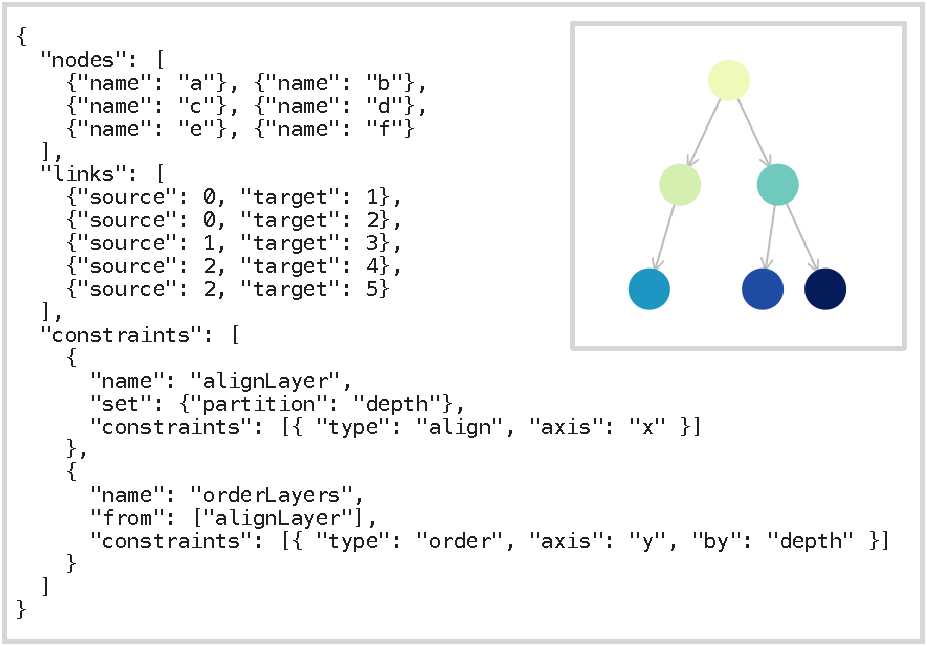
\includegraphics[width=\columnwidth]{figures/small-tree.pdf}
    \vspace{-20px}
    {\caption{\label{fig:small-tree} A simple constraint specification for a tree layout and the resulting layout on a six node tree.}}
  \end{figure}
}